\begin{frame}{Vanishing/Exploding Gradient}
	\begin{itemize}
		\item The issue would be the weight derivatives in Back Propagation.
	\end{itemize}
	\begin{figure}
		\centering
		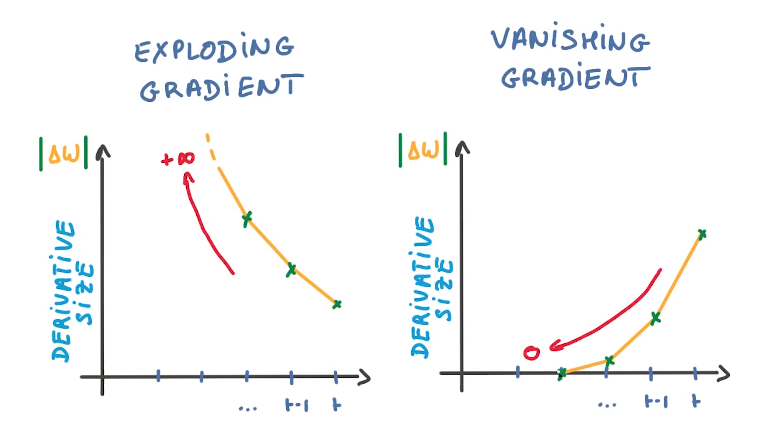
\includegraphics[width=8cm, height=3cm]{Figs/van_2.png}
		\caption{Vanishing/Exploding Gradient, \href{https://medium.com/@ayushch612/vanishing-gradient-and-exploding-gradient-problems-7737c0aa535f}{Source}}
	\end{figure}
\end{frame}

\begin{frame}{Vanishing Exploding Gradient}
	\begin{itemize}
		\item Exploding
		\begin{itemize}
			\item Causes the gradient descent to diverge. 
			\item The model is not learning much on the training data therefore resulting in a poor loss.
			\item Model becomes unstable and give large changes in every update and never leads to the desired model.
		\end{itemize}
	\end{itemize}
\end{frame}

\begin{frame}{Vanishing/Exploding Gradient}
	\begin{itemize}
		\item Vanishing
		\begin{itemize}
			\item Gradient descent never converges to the optimum. 
			\item Model weights shrink exponentially and become very small when training the model.
			\item Make learning slow especially of front layers in the network.
		\end{itemize}
	\end{itemize}
\end{frame}